\section{Multi-Fidelity Gaussian Process Regression} \label{sec:mf_modeling}

It is often the case that simulations or experiments of a sufficiently-high fidelity are too expensive to perform over the entire domain of interest for a modeled problem.
In many cases, there are lower-fidelity approximations available that can be evaluated quickly to perform parameter studies.
The aim of the multi-fidelity GP is to use data from different fidelity levels to create a surrogate model that can best approximate the highest-fidelity function and its uncertainty, while reducing the required number of high-fidelity function evaluations. 

Assume there are $s$ information sources $f_t(\mathbf{x})$, where $t\in\{1,2,...,s\}$, and the function at the highest fidelity level, $f_s(\mathbf{x})$, is being approximated using a Gaussian Processes, $Z_s(\mathbf{x}) \sim \mathcal{N}(\mu_{s}(\mathbf{x}), \sigma_s^2(\mathbf{x}))$.
An auto-regressive formulation of the multi-fidelity framework is used. This was first put forward in \cite{kennedy_predicting_2000} and was improved upon by \cite{gratiet_multi-fidelity_nodate} to reduce computational cost and improve predictions.
The GP approximation at the $t$ fidelity level is modeled as

\begin{equation}
    Z_t(\mathbf{x}) = \rho_{t-1}(\mathbf{x})Z_{t-1}(\mathbf{x}) + \delta_t(\mathbf{x}),
\end{equation}
\begin{equation}
    \rho_{t-1}(\mathbf{x}) = \mathbf{g}_{t-1}^T(\mathbf{x})\beta_{\rho_{t-1}},
\end{equation}
where $\mathbf{g}_{t-1}(\mathbf{x})$ is a set of $q$ basis functions, similar to $\mathbf{h}(\mathbf{x})$ in the previous section, $\beta_{\rho_{t-1}}$ is the learned regression coefficients, and $\delta_t(\mathbf{x})$ is modeled using a GP.
A way to interpret these terms is to consider $\delta_t(\mathbf{x})$ the additive bias and $\rho_{t-1}(\mathbf{x})$ the multiplicative bias between fidelity levels $t$ and $t-1$.
To account for the different fidelity levels and their corresponding data, the subscript $t$ is added to the notation introduced in Section \ref{sec:gpr}.
For example, $X_t$ refers to all the input data at level $t$. Additionally, the term $\Sigma_t = \text{diag}(\sigma^2_{i,t})$ is introduced, which refers to the noise in the outputs $\mathbf{y_t}$. 

In Appendix B of \cite{gratiet_multi-fidelity_nodate}, Gratiet presents the predictive equations for the case when the design sets are not nested ($\mathcal{D}_t \notin \mathcal{D}_{t-1}$) and the data has no process noise, such that $\Sigma_t$ is a null matrix.
This work extends those equations to include process noise $\Sigma_t \neq \emptyset$, which produces the following representations for the mean and covariance equations for fidelity level $t \neq 1$ as

\begin{equation}\label{equ:mu_Zt}
\begin{split}
    \mu_{t}(X_*) = & ~ \rho_{t-1} \left ( X_* \right ) \mu_{t-1} \left (X_* \right ) + H_*^T\beta_t \\
    & + \left [ \left ( \rho_{t-1} \left (X_* \right ) \rho_{t-1} \left (X_t \right )^T \right ) \odot \sigma^2_{t-1} \left(X_*,X_t \right) + K_{t} \left(X_*,X_t \right)\right] \\ 
    & \times \left [ \left ( \rho_{t-1} \left (X_t \right ) \rho_{t-1} \left (X_t \right )^T \right ) \odot \sigma^2_{t-1} \left(X_t,X_t \right) + V_t \right ]^{-1} \\ 
    & \times \left (\mathbf{y}_t - \rho_{t-1} \left (X_t \right ) \odot \mu_{t-1} \left (X_t \right) - F_t^T \beta_t \right),
\end{split}
\end{equation}
and
\begin{equation}\label{equ:sig_Zt}
\begin{split}
    \sigma^2_{t}(X, \Tilde{X}) = & ~ \left (\rho_{t-1} \left ( X \right ) \rho_{t-1} ( \Tilde{X})^T \right ) \odot \sigma^2_{t-1} (X, \Tilde{X}) + K_t(X, \Tilde{X}) - \\
    & \left [ \left ( \rho_{t-1} \left (X \right ) \rho_{t-1} \left (X_t \right )^T \right ) \odot \sigma^2_{t-1} \left(X,X_t \right) + K_{t} \left(X,X_t \right)\right] \\ 
    & \left [ \left ( \rho_{t-1} \left (X_t \right ) \rho_{t-1} \left (X_t \right )^T \right ) \odot \sigma^2_{t-1} \left(X_t,X_t \right) + V_t \right ]^{-1} \\ 
    & \left [ \left ( \rho_{t-1} \left (X_t \right ) \rho_{t-1} ( \Tilde{X} )^T \right ) \odot \sigma^2_{t-1} (X_t, \Tilde{X} ) + K_{t} ( X_t, \Tilde{X} ) \right], 
\end{split}
\end{equation}
where $(X, \Tilde{X})$ are generic input arguments, $V_t = K_{t} \left(X_t,X_t \right) + \Sigma_t $, and $\rho_{t-1} (X) = G_{t-1}(X)^T \beta_{\rho_{t-1}}$.
$G_{t-1}(X)$ is a $q \times n$ matrix where each column is a $q$-dimensional result of the basis functions for the corresponding $m$-dimensional row of input samples in $X$, and $\beta_{\rho_{t-1}}$ are learned regression coefficients.
For the lowest fidelity level, $t=1$, the regular GP regression equations, Equations \ref{equ:mu_gpr} and \ref{equ:sig_gpr}, are used.
For a set of sample locations $X_*$, the mean predictions at fidelity level $t$ is given by $\mu_t(X_*)$ and the variance in the predictions is given by the diagonal of $\sigma^2_t(X_*,X_*)$. 

To fully define the GP of each fidelity level, the regression coefficients ($\beta_{\rho_{t-1}}$ and $\beta_t$) and the hyperparameters of the kernel functions of each fidelity level need to be learned from the data.
The parameter estimation equations from  \cite{gratiet_multi-fidelity_nodate} are extended for noisy observations:

\begin{equation}
    \begin{bmatrix}
    \beta_t & \beta_{\rho_{t-1}}
    \end{bmatrix} = \left [ J_t^T \left ( K_t(X_t,X_t) + \Sigma_t \right )^{-1} J_t \right ]^{-1} \left [ J_t^T \left ( K_t(X_t,X_t) + \Sigma_t \right ) ^{-1} \mathbf{y_t} \right ], 
\end{equation}
with $J_1 = H_1$ and for $t > 1$, $J_t =  \begin{bmatrix} G_{t-1} \odot \left ( \mu_{t-1} \left ( X_t \right )  \mathbf{1}_{q_{t-1}} \right ) & F_t \end{bmatrix}$.
$\mathbf{1}_{q_{t-1}} \in \mathbb{R} ^{q_{t-1} \times n_t} $ is a matrix of ones.
The hyperparameters of the kernel functions are learned by minimizing the negative marginal log-likelihood of each fidelity level.

\begin{equation}
    \log~p(\mathbf{y}_t|X;\theta) = -\left (\frac{1}{2} \log|V_t| + \frac{1}{2} \alpha^T V_t^{-1} \alpha + \frac{n_t}{2}\log 2\pi \right),
\end{equation}
where $\alpha = \left (\mathbf{y_t} - \rho_{t-1} \beta_{\rho_{t-1}}-F_t\beta_t \right )$.

To show the potential advantage of using multi-fidelity data to estimate a function of interest, the analytic functions defined by Equations \ref{equ:lf_function} and \ref{equ:hf_function} are used as the low-fidelity approximation and the high-fidelity function of interest respectively. 
For this case, the number of high-fidelity data points is restricted to $4$. 
Figure \ref{subfig:sf_gpr} shows the mean and error estimates for a one-fidelity GP trained on just the 4 high-fidelity data points. 
$\sigma_i^{HF} = 0.3$ in this case.
There aren't enough data points for the GP regression to learn all the nuanced trends in the high-fidelity function of interest. 
For Figure \ref{subfig:mf_gpr}, the low-fidelity function (yellow line) is introduced by using 11 equally spaced function evaluations (blue squares). 
The low-fidelity data doesn't have some of the higher-frequency information that is present in the high-fidelity data, but it approximates the general trends fairly well. 
In this case, the low-fidelity data bolsters the scant $4$ high-fidelity data points, and the multi-fidelity GP that combines both sets of data, is able to provide a more accurate representation of the underlying function of interest. 
It is also important to notice the large error estimates in GP prediction. 
More high-fidelity data would be required to reduce the uncertainty in the GP modeling. 

\begin{figure}
    \centering
    \begin{subfigure}[\label{subfig:sf_gpr} Single-fidelity fit.] {
        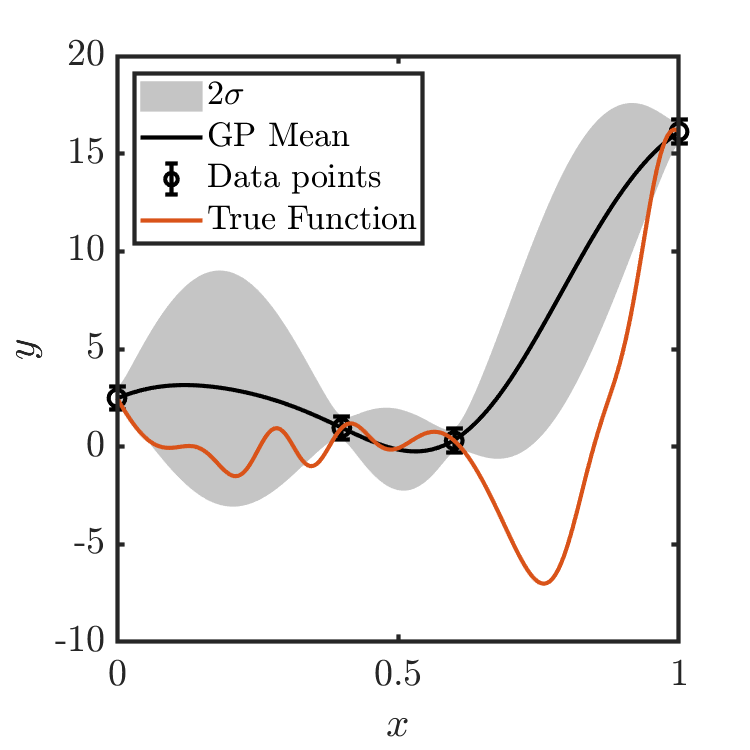
\includegraphics[width=.45\textwidth]{code/image_gen/gp_analytical/images/hf_4_noise.png} }
    \end{subfigure}
    \hfill
    \begin{subfigure}[\label{subfig:mf_gpr} Two-fidelity fit.]{
        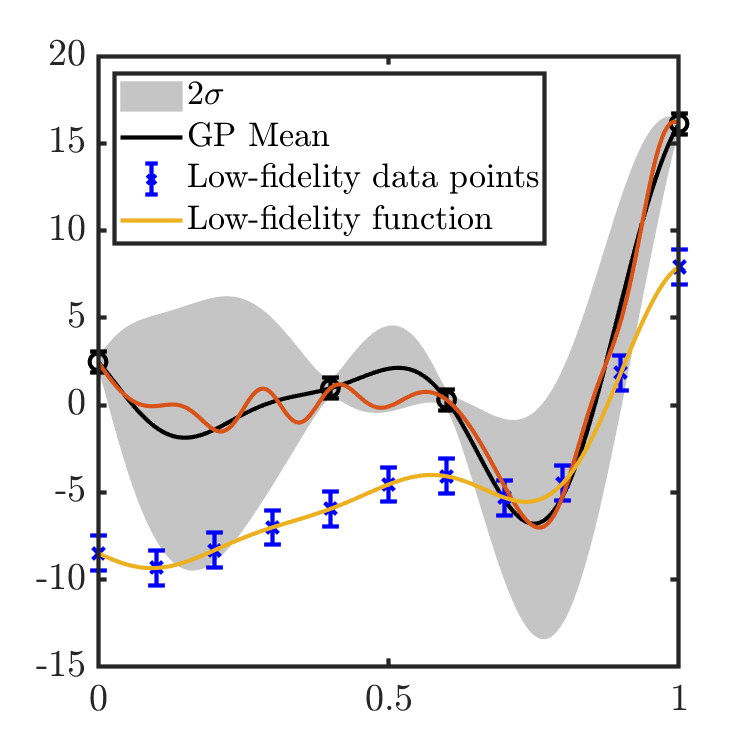
\includegraphics[width=.45\textwidth]{code/image_gen/gp_analytical/images/mf_4_noise.png} 
    }
    \end{subfigure}
    \caption{Comparison of single- and two-fidelity GP regression. \label{fig:mf_vs_sf_analytic}}
\end{figure}

As mentioned earlier in this section, the recursive formulation put forth by Gratiet \cite{le_gratiet_recursive_2014} improves on the work originally done by Kennedy and O'Hagan \cite{kennedy_predicting_2000} by reducing the computational complexity of the training and sampling steps of the multi-fidelity GP.
This is achieved by splitting the dataset into each individual fidelity level instead of agglomerating the data from all levels into one set of equations.
This results in having to invert smaller matrices, which greatly improves the computational cost of the process.
Figure \ref{fig:time_comp} shows the comparative times for the training and sampling steps. 
The same analytic functions used thus far, Equations \ref{equ:lf_function} and \ref{equ:hf_function}, are used to train the GP regressions.
In this case, the number of high-fidelity data points ($n_{HF}$) and low-fidelity data points ($n_{LF}$) had a constant ratio: $\frac{n_{HF}}{n_{LF}} = 0.2$.
These savings in computational time increase with more fidelity levels and higher-dimensional functions. 

\begin{figure}
    \centering
    \begin{subfigure}[Time taken to train the multi-fidelity GP.] {
        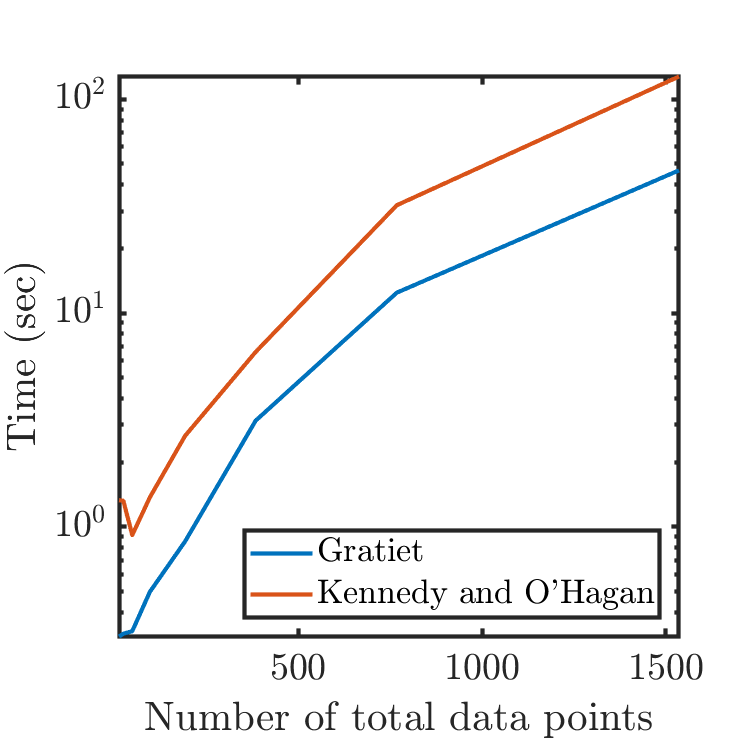
\includegraphics[width=.45\textwidth]{code/image_gen/gp_analytical/images/time_process.png} }
    \end{subfigure}
    \hfill
    \begin{subfigure}[Time taken to sample the multi-fidelity GP.]{
        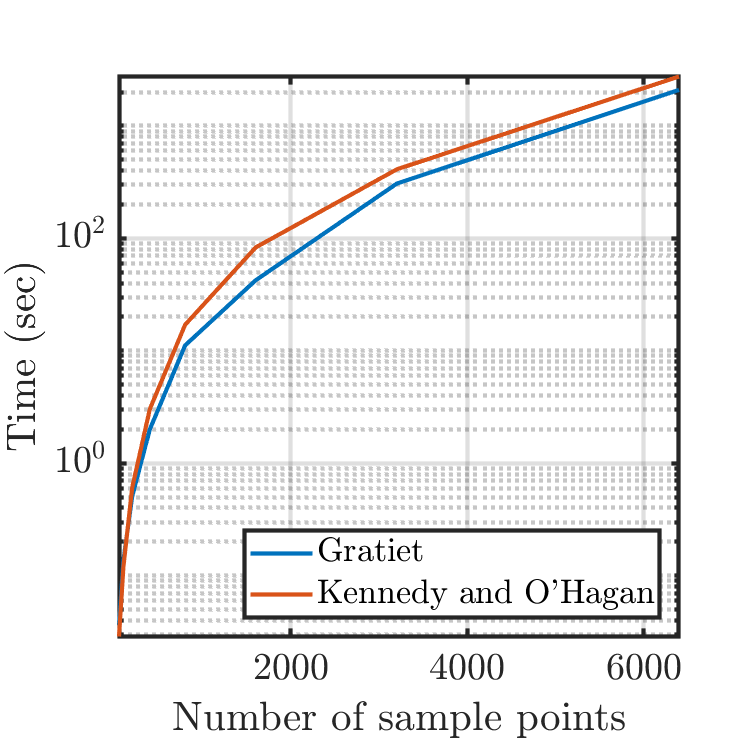
\includegraphics[width=.45\textwidth]{code/image_gen/gp_analytical/images/time_query.png} 
    }
    \end{subfigure}
    \caption{Wall clock time comparison to train and query the multi-fidelity Gaussian Process formulations put forth by Kennedy and O'Hagan \cite{kennedy_predicting_2000}, and Gratiet \cite{gratiet_multi-fidelity_nodate}. \label{fig:time_comp}}
\end{figure}